\documentclass[utf8]{webofc}
\usepackage[varg]{txfonts}
% review
\usepackage[textwidth=120]{todonotes}
%\usepackage{color}
\usepackage{subcaption}

\begin{document}
    \title{About some question in modern models of thunderstorm runway breakdown}
    \author{\firstname{Mikhail} \lastname{Zelenyi}\inst{1,2,3}\fnsep\thanks{\email{mihail.zelenyy@phystech.edu}} \and
        \firstname{Egor} \lastname{Stadnichuk}\inst{1,2}\fnsep\thanks{\email{egrstadnichuk@yandex.ru}} \and \firstname{Alexander} \lastname{Nozik}\inst{1,2}\fnsep\thanks{\email{altavir@gmail.com}}  
    }
    
    \institute{Institute for Nuclear Research of RAS
        \and
        Moscow Institute of Physics and Technology (State University) 
        \and
        Space Research Institute of RAS
    }
    \abstract{%
        Some of modern models used to describe TGF phenomena and lightning ignition suppose the existence of the positive positron or gamma ray feedback. The results of Monte-Carlo simulation, presented in this work encourage to give a fresh look into this problem. Namely, the positive enhancement for experimentally observed electric fields in thunderclouds is not enough to produce positive feedback.
        %In modern models based on runway breakdown and created for explaining initiation of lighting and TGF phenomenon, there has been a strong emphasis on peak of positron annihilation in observed gamma-ray spectra. This observation used as evidence importance of positron feedback in thunderstorms. But in this report, we give some result of Monte-Carlo simulations speaking about weak influence of positrons on thunderstorm processes and appearance of TGF.
    }
    %
    \maketitle
    
    \section{Introduction}
    Despite decades of investigations and observations, there are gaps in physics of atmospheric discharge. Nowadays the process of development of lightning after initial breakdown is widely known. However, the mechanism of cloud ionization which is required to produce initial breakdown is not described accurately. Furthermore, some observed effects connected to lightning generation also lack explanation. For example, terrestrial gamma ray flashes (TGFs) are closely correlated with thunderstorms. This phenomenon has several explanations but none of them are considered satisfying.
    \begin{figure}[ht!]
        \begin{subfigure}[b]{0.5\textwidth}
            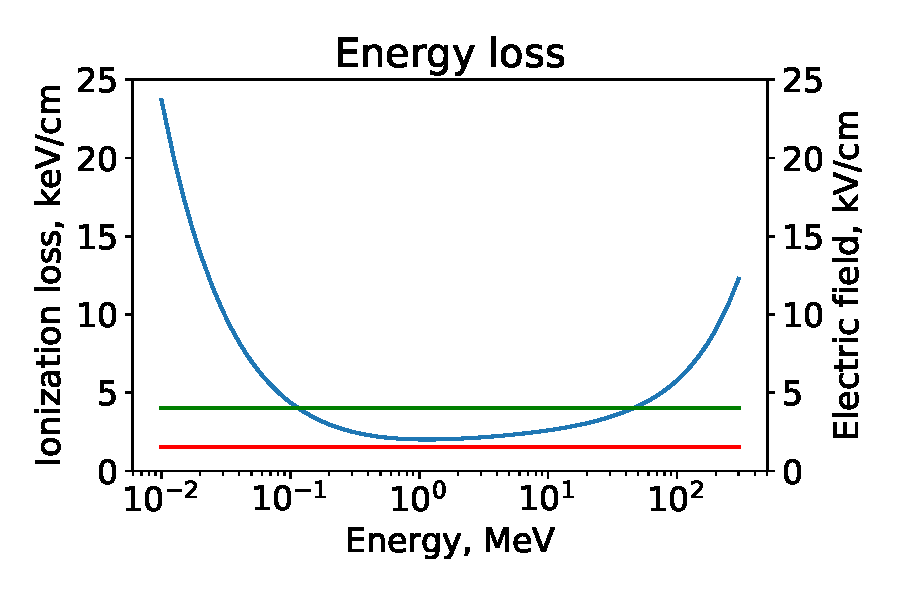
\includegraphics[width=0.95\linewidth]{pictures/01_Gurevich}
            \caption{}
            \label{pic-gurevich-a}
        \end{subfigure}
        ~
        \begin{subfigure}[b]{0.5\textwidth}
            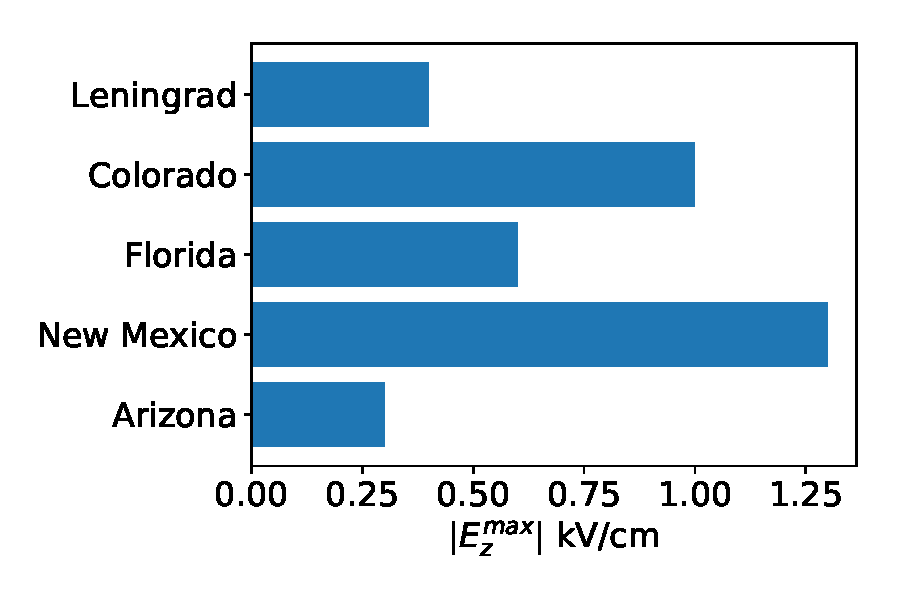
\includegraphics[width=0.95\textwidth]{pictures/03_extremal_field}
            \caption{}
            \label{pic-field-b}
        \end{subfigure}
        \caption{
            a) Gurevich model: if electric field higher than MIP loss (green line) that possibly generation runway electron, otherwise (red line) avalanches discharged~\cite{gurevich1992runaway}.
            %     a) Distribution of horizontal electric field ~\cite{mazin1989clouds} 
            b) Extremal value of vertical electric field (before 1989 y.)~\cite{mazin1989clouds}}
    \end{figure}
    
    Gurevich has made a notable contribution in understanding of electron avalanche physics in atmosphere~\cite{gurevich1992runaway}. According to his research, cosmic ray charged particles are accelerated in thundercloud electric field and are producing enhanced ionization. Gurevich studied electron behavior in air with electric field. Energetic electrons that are able to accelerate under such conditions are called runaway electrons (see Fig. ~\ref{pic-gurevich-a}). In the following works, Gurevich developed the runaway theory~\cite{gurevich1999lightning,gurevich2001kinetic}. Nevertheless, the flux of cosmic rays is not intensive enough to explain cloud charging with only runaway electron ionization.
    Dwyer proposed a mechanism of positron feedback that increases the runaway electron flux ~\cite{dwyer2003fundamental}. Dwyer constructed his simulation in the cell with electric field value of 1000 kilovolt per meter. A cell is a cylinder of air with electric field. Dwyer’s feedback mechanism is described briefly as follows. A runaway electron propagating through such a cell radiates bremsstrahlung photons. If the bremsstrahlung photon has enough energy, then it can produce an electron-positron pair. The positron charge is opposite to the electron charge, therefore it reverses in electric field and then propagates in direction opposite to the runaway electron motion direction. Such positrons have a chance to produce electrons near the beginning of primary runaway electron track. Then ionization electrons can reverse in the electric field and propagate through cell creating secondary electron avalanche. The runaway theory with Dwyer feedback mechanism is considered to be one of the most reliable theories describing processes appearing in thunderclouds before lightning strike. Example of Dwyer mechanism is shown at Fig.~\ref{pic-dwyer-a}.
    
    Direct measurements show that observed thundercloud electric field is less than 200 kilovolts per  meter(~\cite{mazin1989clouds, marshall1995electric}). Some data points are showed at Fig.~\ref{pic-field-b}. However, there are no results in literature regarding how positron feedback works under such conditions. The aim of the present work is to reveal whether Dwyer model operates in cells with uniform electric field less than 200 kilovolts per meter and air density between 0.3 and 0.8 kilogram per cubic meter and to calculate positron feedback coefficients for different electric fields. %The algorithm of feedback coefficient calculating is described in methodology section.
    %The results of the investigation are negative. The paper shows that positron feedback coefficient is much less than 1 in cells with electric field under 200 kilovolts per meter. That means that one electron avalanche does not create secondary avalanches by positron feedback mechanism. The accurate value of positron feedback coefficient is stated in results section.
    
    \newsavebox{\leftpic}
    \begin{figure}[t]\centering
        % Левая картинка (а) помещена в бокс, чтобы измерить её высоту
        \sbox{\leftpic}%
        {% Левая картинка (a):
            \begin{subfigure}[b]{0.4\linewidth}\centering
                %height=7cm]
                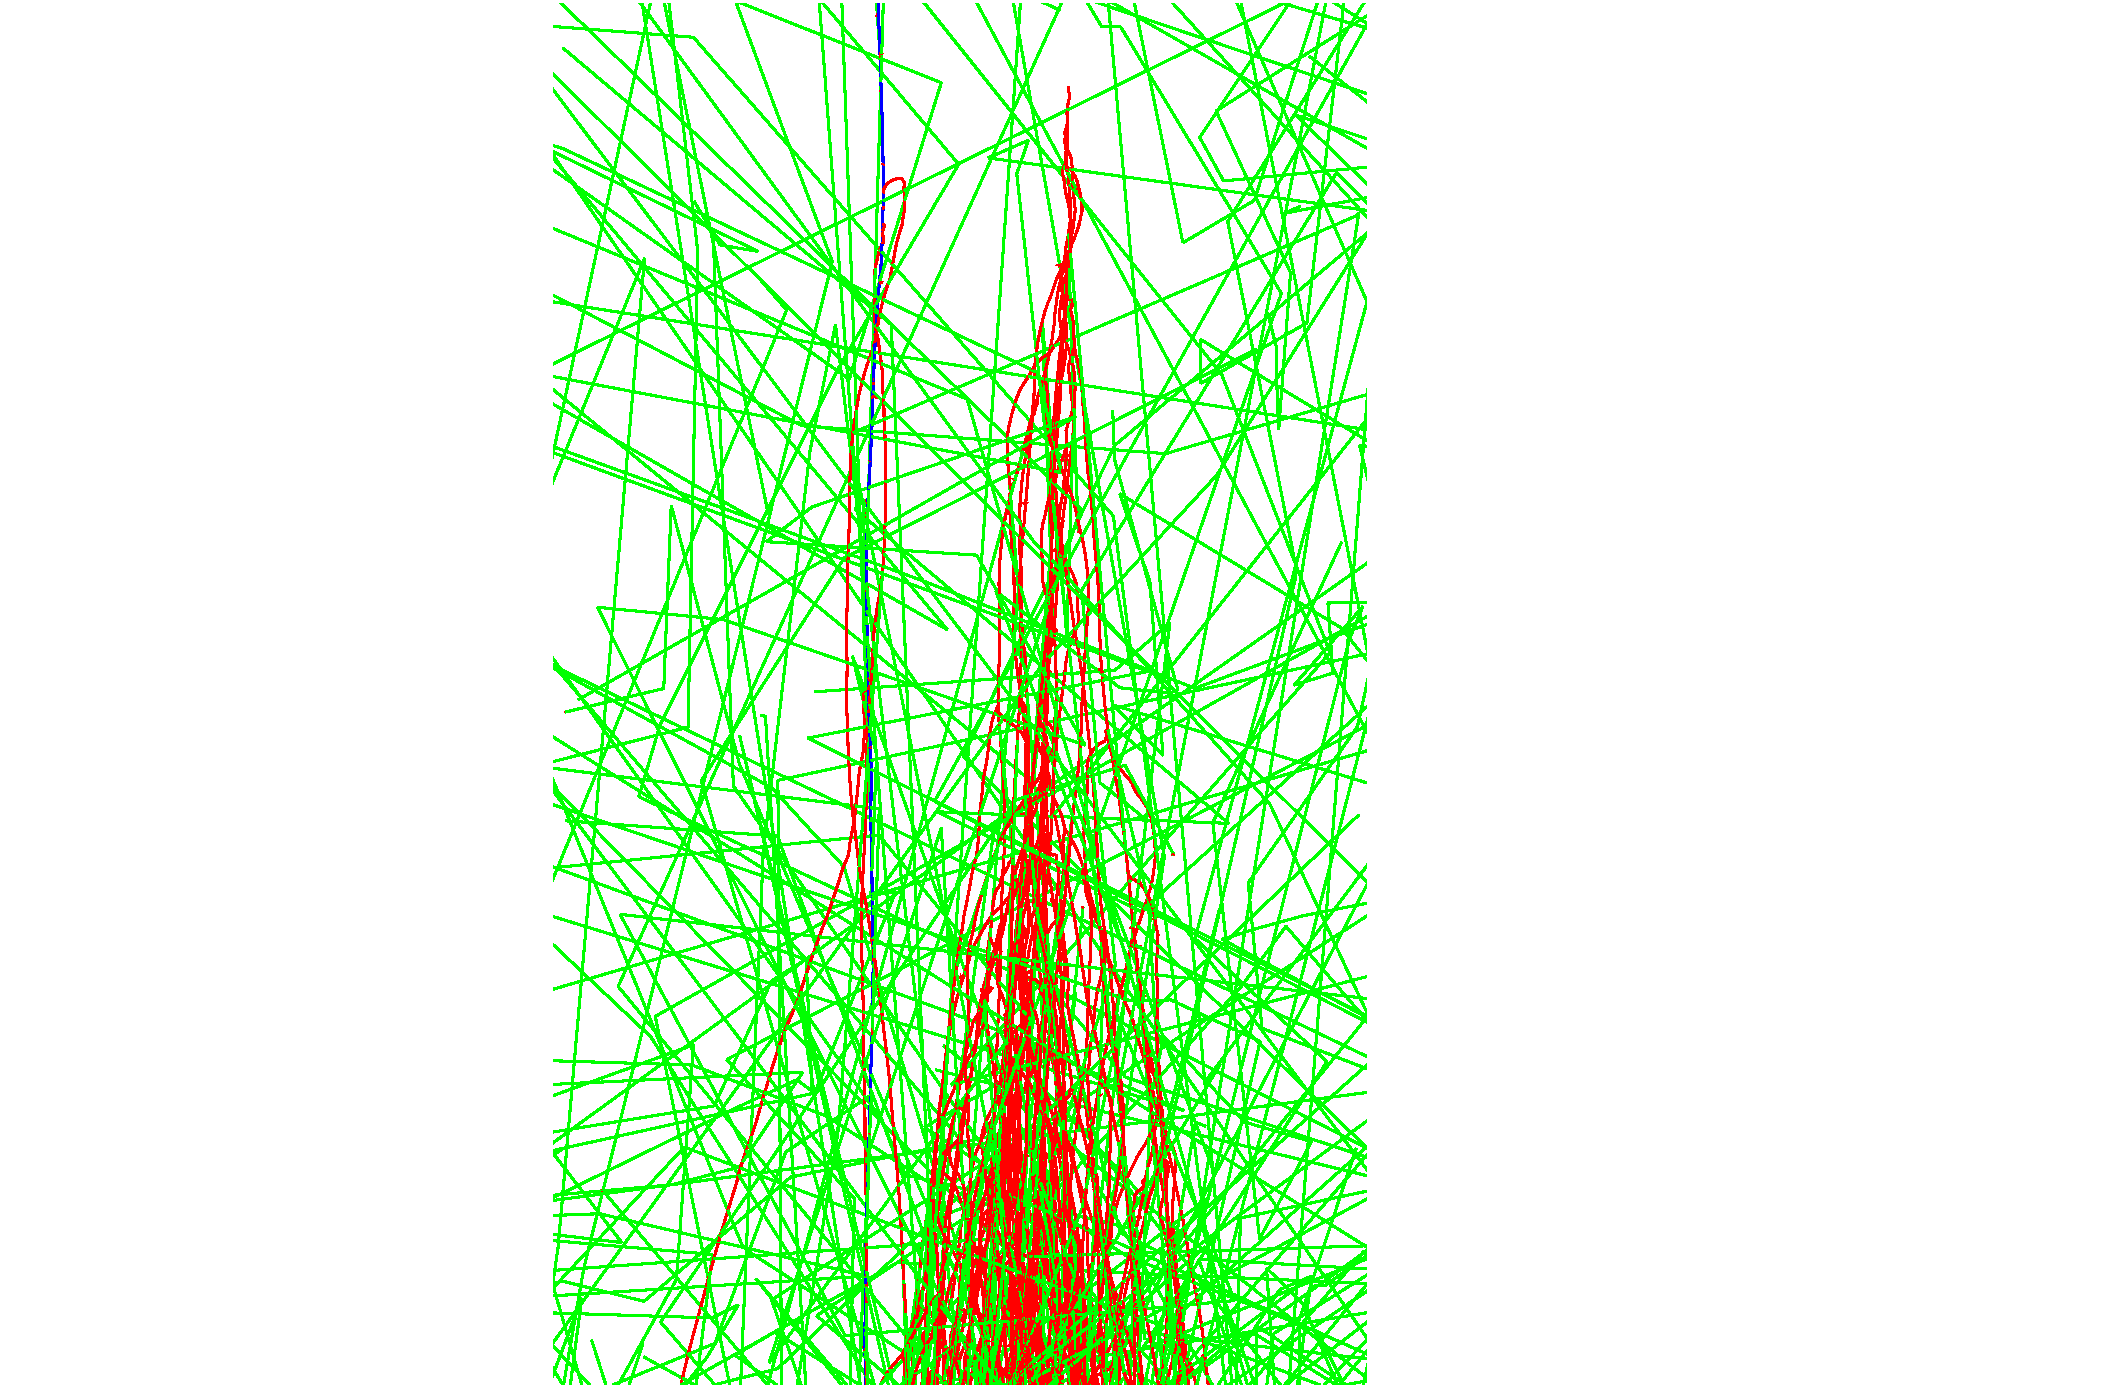
\includegraphics[width=0.95\textwidth]{pictures/10_dwyer}
                \caption{}\label{pic-dwyer-a}
            \end{subfigure}%
        }
        %------------------------
        % Вывысти картинку, сохраненную в боксе
        \usebox{\leftpic}
        \quad % немного пустого места между левой и правой картинками
        % Две правые картинки в минипейдж, 
        %   - высота которого равна высоте левой картинки: \ht\leftpic
        %   - материал будет растянут вертикально: [s] + \vfill 
        \begin{minipage}[b][\ht\leftpic][s]{0.5\linewidth}
            \begin{center}
                \begin{subfigure}[b]{\textwidth}
                    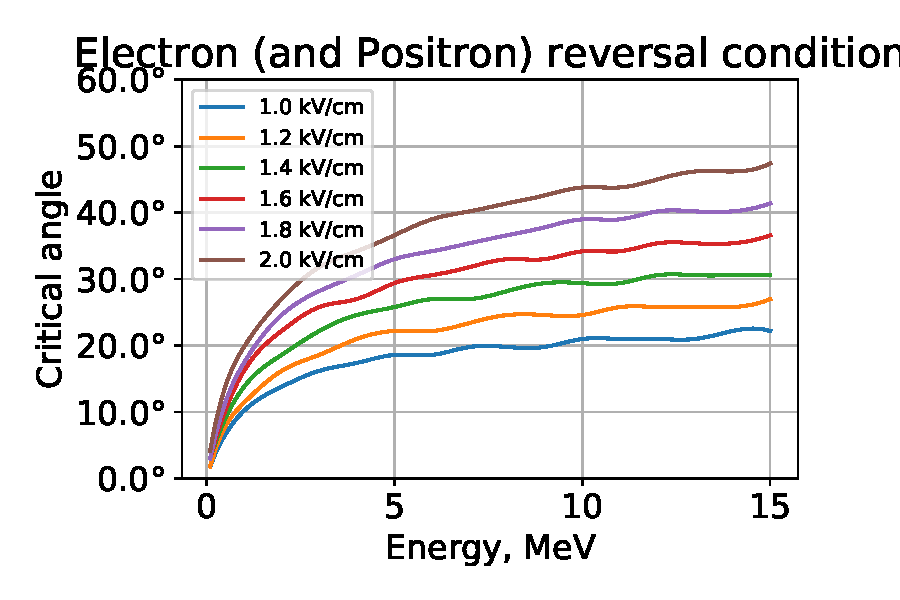
\includegraphics[width=0.9\textwidth]{pictures/09_condition}
                    %\captionof{subfigure}{}
                    \caption{}
                    \label{pic-reverse-b}
                \end{subfigure}
                
            \end{center}      
            \vfill
            
            \begin{center}
                %height=2.5cm
                \begin{subfigure}[b]{\textwidth}
                    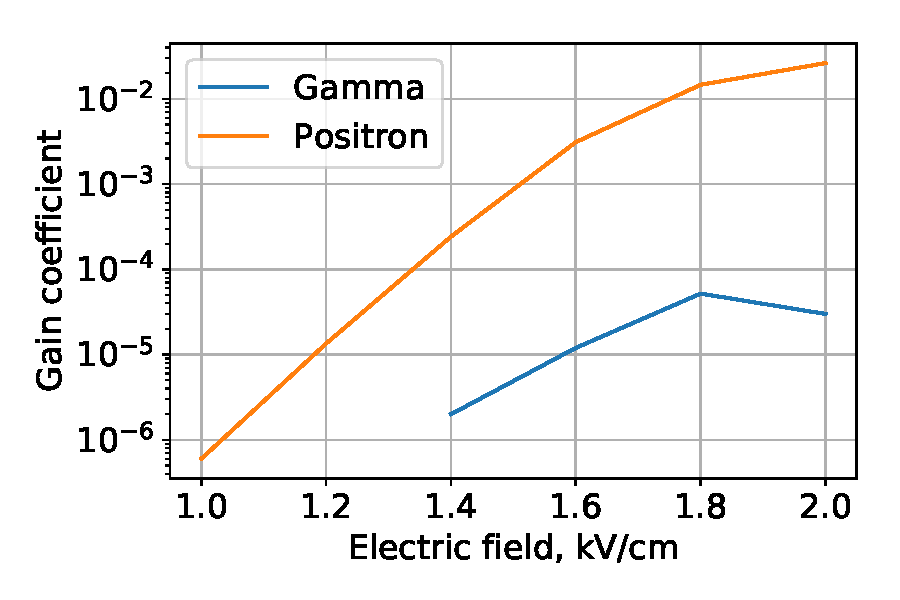
\includegraphics[width=0.85\textwidth]{pictures/08_gain}
                    %\captionof{subfigure}{}
                    \caption{}
                    \label{pic-gain-a}
                \end{subfigure}
                
            \end{center}
        \end{minipage}
        \caption{ a) Part of Geant 4 simulation. Red tracks – electrons. Blue tracks – positrons. Green tracks - gamma-rays. Simulation conducted for normal air density and electric field 10 kV/cm. Left blue track is positron which generate new runway avalanche and illustrate positron feedback mechanism.
            b) Minimum reversal angle between electron motion direction in moment of its birth and electric field depending on electron energy. All of electrons situated above the curve are able to generate secondary electron avalanche in the cell. According to this graph, less than 50\% of electrons produced by positrons will generate secondary electron flux.
            c) Positron (gamma) feedback coefficient dependent on cell electric field for next parameters: primary electron energy - 3 MeV, field area size - 400 meter, electric field from 1 to 2 kV/cm, air density - $0.5~kg/m^3$ ($\sim 0.5~atm$).
        }    
    \end{figure}
    
    \section{Simulation}
    %Aim of our research is estimate of coefficient of reproduction (gain) for gamma and positron feedback. 
    In this work we consider two mechanisms proposed by Dwyer: gamma feedback and positron feedback. 
    In both cases the idea is similar:
    \begin{enumerate}
        
        \item Initial electron accelerates in the electric field and produces photon which is flying backwards or positron which is reversed by electric field and also flies backward.
        
        \item The positron or photon produces electron near the beginning of the acceleration cell.
        
        \item This electron is rotated by the electric field and produces the secondary avalanche. 
        
    \end{enumerate}
    
    The electron produced in the last phase is called secondary electron. The gain coefficient is defined as an average number of secondary electrons produced per single initial electrons. Obviously, in order to have significant enhancement mechanism, one need gain to be greater or equal to 1. 
    The gain is obviously proportional to the number of positrons and/or gamma rays generated by initial electron, but there is a number of factors that contribute to that quantity.
    
    \begin{itemize}
        \item Positrons are mostly produced not directly, but by bremsstrahlung gamma rays emitted by initial electron. The mean free path of this gamma for this process is quite large (of the order of few kilometers for atmospheric conditions). Therefore, the probability of generating positron inside the acceleration cell is proportional to cell size and density (increase in density reduces the mean free path). Also, the number of positrons is proportional to field in cell (since electrons with higher energy are more likely to produce appropriate photons).
        \item Not all positrons are accelerated backwards. Due to conservation of momentum, large fraction of them are moving forward. Those positrons are usually stopped by electric field and annihilated.
        \item Accelerated positron has rather small probability to directly produce an electron because the cross-section diminishes with energy.
        \item Secondary electrons, produced both by positrons and gamma rays are usually fly toward "back" side of the cell due to conservation of momentum. Those electron could be rotated by the electric field to fly forward, but one must remember, that once electron energy is below Gurevitch's critical energy, it could not be accelerated and is lost.
    \end{itemize}
    
    The simulation are done by GEANT4 transport code (\cite{ALLISON2016186}) in three steps:
    
    \begin{enumerate}
        \item Calculate energy and angular spectra of positrons and gamma rays of sufficient energy, which are produced inside the cell.
        \item Use those spectra as initial distributions for secondary simulation of particles flying backwards and register all secondary electrons.
        \item Select only those electrons, which could be later reversed forward without stopping. Minimal particle energy is determined from value of electric field and ionization loss curve (~\ref{pic-gurevich-a}). The dependence of minimal angle between cell axis backward direction and velocity is shown at Fig.~\ref{pic-reverse-b}
    \end{enumerate}
    
    
    %We define gain coefficient for feedback as a ratio between the number of secondary electron, generating from positron (gamma) feedback and number of primary electron. We count only those secondary electrons that are potentially able to create secondary avalanche. Specifically, they are born near the "top" side of the cell and have momentum directed in direction of the breakdown. Then avalanches, generating this electron, will keep in area with electric field and will participate in runway breakdown.
    
    % \todo{Вот тут надо поподробнее. Что именно считается вторичными электронами. З. Добавил} 
    % For define gain coefficient, we conduct simulation using Geant4 transport code~\cite{ALLISON2016186}. In order to improve performance we split our simulation on two parts:
    % \begin{itemize}
    % 	\item First, we compute spectra of positrons and gamma-rays in avalanche for different energies of primary electron and select only those positrons and gamma-rays that could produce secondary backward avalanches;
    % %     \todo{надо наверное добавить backward?}
    
    % 	\item Secondly, we compute spectrum of secondary electron created by positrons and gamma-rays and select those electron that could produce new avalanches.
    
    % \end{itemize}
    
    % As rule for validation of particle we use two condition:
    % \begin{itemize}
    
    %     \item Particle energy is higher than runway energy~\cite{gurevich1992runaway}. 
    % %     \todo{ссылку или объяснение по поводу того, что это такое. З. Добавил ссылку}.
    
    % 	\item If positron (electron) have momentum to direct against (on) electric field, then its energy and angle should allow it to be reversed in electric field without stopping. 
    % %     \todo{как-то мутно тут. У нас же две вторичных частицы. Одна летит назад, другая потом вперед. Про какую из них речь. З. Добавил}.
    
    % \end{itemize}
    
    % Then gain coefficient is produced by following formula:
    % \begin{equation*}
    % 	\label{eq-gain}
    % 	\gamma_{e^+, \gamma} = \int N_{e^+, \gamma}(E_{pr},P_{e^+, \gamma}) 
    %     N_{e^-}(P_{e^+, \gamma}, P_{e^-})
    %     I[E_{e^+, \gamma}, E_{e^-} > E_{rw}] I[\theta_{e^-, e^+} > \theta_{c}]
    %     ~dE_{pr}~dP_{e^+, \gamma}~dP_{e^-},
    % \end{equation*}
    % where $N_{e^+, \gamma}$ --- number of positrons (gamma-quanta) with four-momentum $P_{e^+, \gamma}$ per primary electron with energy $E_{pr}$, $N_{e^-}$ --- number new primary electron with four-momentum $P_{e^-}$ per positron (gamma-quantum), $E_{rw}$ --- energy of runway, $\theta_{e^-, e^+}$ --- angle between particle and electric field directions, $\theta_c$ --- critical angle of reversal in electric field,   $I[condition]$ is $1$ if condition is true and $0$ otherwise.
    
    \section{Results}
    
    % \begin{figure}[ht!]
    % 	\begin{subfigure}[b]{0.5\textwidth}
    %     	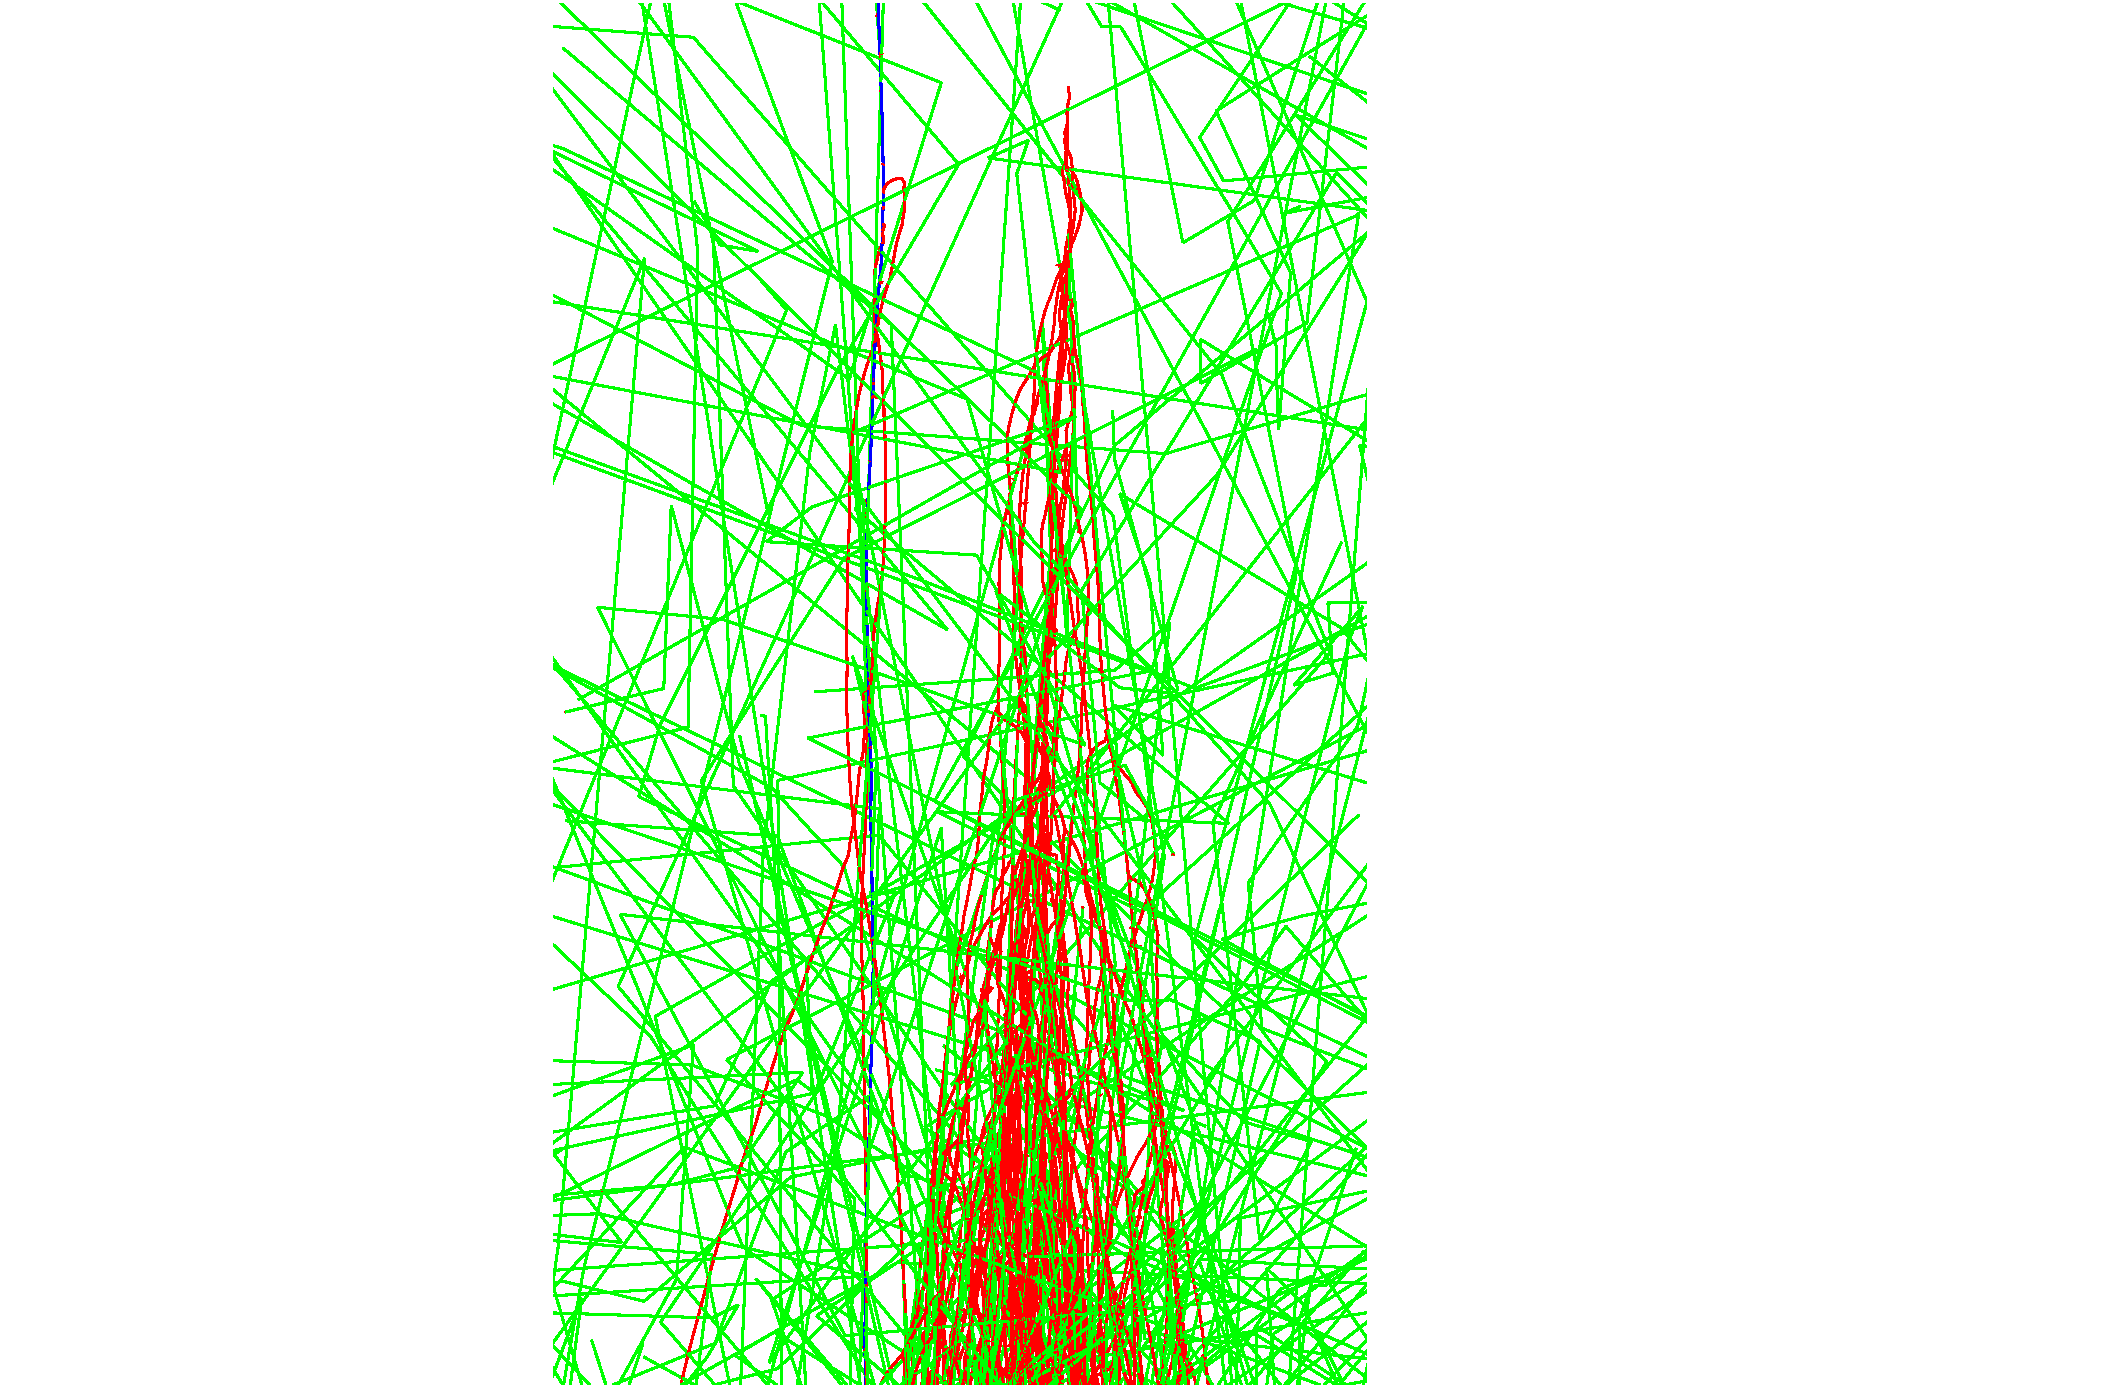
\includegraphics[width=0.95\linewidth]{pictures/10_dwyer}
    %         \caption{}
    %         \label{pic-dwyer-a}
    %     \end{subfigure}
    % 	~
    %     \begin{subfigure}
    %         \begin{subfigure}[b]{0.22\textwidth}
    % 		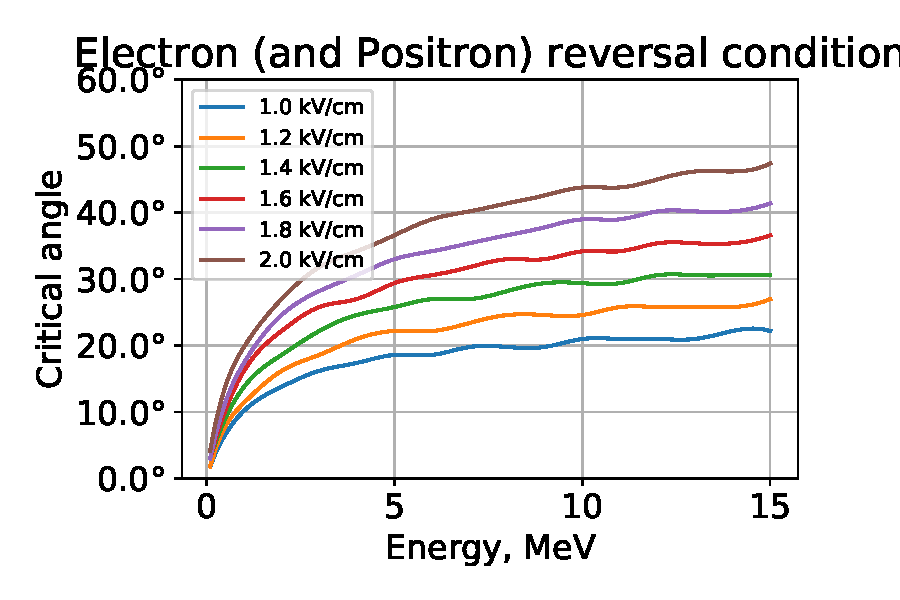
\includegraphics[width=0.95\textwidth]{pictures/09_condition}
    %         \caption{}
    %         \label{pic-reverse-b}
    %     \end{subfigure}
    %     ~
    %       \begin{subfigure}[b]{0.22\textwidth}
    % 		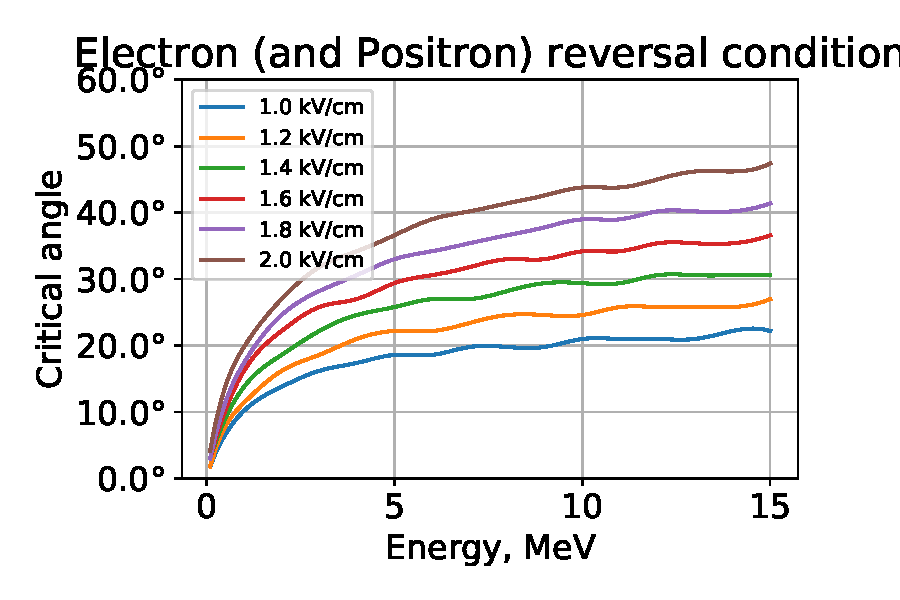
\includegraphics[width=0.95\textwidth]{pictures/09_condition}
    %         \caption{}
    %         \label{pic-reverse-b}
    %     \end{subfigure}
    %     \end{subfigure}
    
    %     \caption{
    % %     a) Gurevich model: if electric field higher than MIP loss (green line) that possibly generation runway electron, otherwise (red line) avalanches discharged. 
    %     a) Dwyer model in Geant 4 simulation. Red tracks – electrons. Blue tracks – positrons. Green tracks - gamma-rays
    %     b) Minimum reversal angle between electron motion direction in moment of its birth and electric field depending on electron energy. All of electrons situated above the curve are able to generate secondary electron avalanche in the cell. According to this graph, less than 50\% of electrons produced by positrons will generate secondary electron flux}
    % \end{figure}
    
    %Minimal particle energy is determined from value of electric field and ionization loss curve (~\ref{pic-gurevich-a}). Particles ability to turn in electric field are calculated in dry friction model where average ionization energy loss used as  a friction force, bremsstrahlung are not taken into account due to its small effect compared to ionization losses. From this model, for every energy, we get critical angle between field and particle momentum direction, at which particles couldn't reverse in the field. As example, Fig. ~\ref{pic-reverse-b} shows critical angle for cloud at height 8 km.
    
    % \begin{figure}[ht!]
    % 	\begin{subfigure}[b]{0.5\textwidth}
    %     	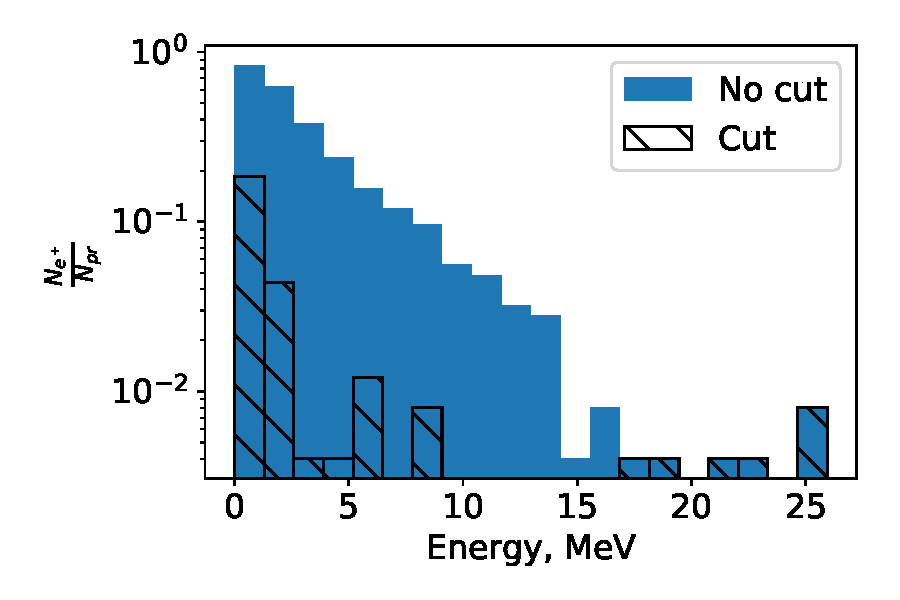
\includegraphics[width=0.95\linewidth]{pictures/04_energy_cut_positron}
    %         \caption{}
    %         \label{pic-positron-cut-a}
    %     \end{subfigure}
    % 	~
    %     \begin{subfigure}[b]{0.5\textwidth}
    % 		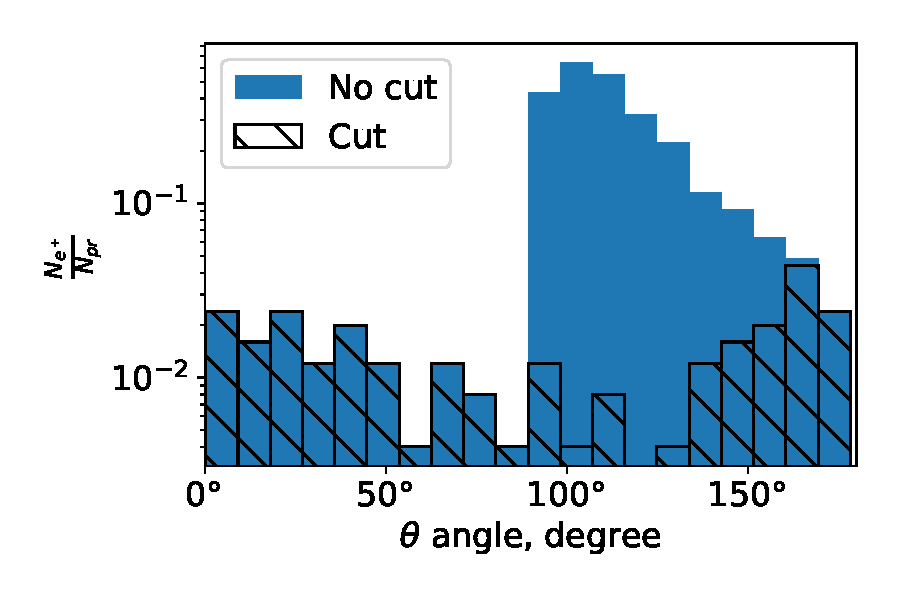
\includegraphics[width=0.95\textwidth]{pictures/05_theta_cut_positron}
    %         \caption{}
    %         \label{pic-positron-cut-b}
    %     \end{subfigure}
    %     \caption{ a) Energy b) polar angle positron distribution after and before cut for next parameters: primary electron energy - 1 MeV, field area size - 400 meter, electric field 2.5 kV/cm, air density - $0.5 kg/m^3$ ($\sim 0.5 atm$)}
    % \end{figure}
    
    % % \todo{Вообще не понял, что это и на каком языке}
    % % Переход от следующего пункта, там мы посчитали условия, а здесь мы счиатем спекрты для разных наборов параметров
    % Further, we calculate positron, gamma and secondary electron spectra. In simulation we consider cylindric area with different parameters set: electric field under $2.5 kV/cm$, air density between $0.3$ and $0.8 kg/m^3$ (clouds height from 4 to 12 km), field area size  200-400 meters, primary electron energy between 1 and 10 MeV.
    
    % \begin{figure}[ht!]
    % 	\begin{subfigure}[b]{0.5\textwidth}
    %     	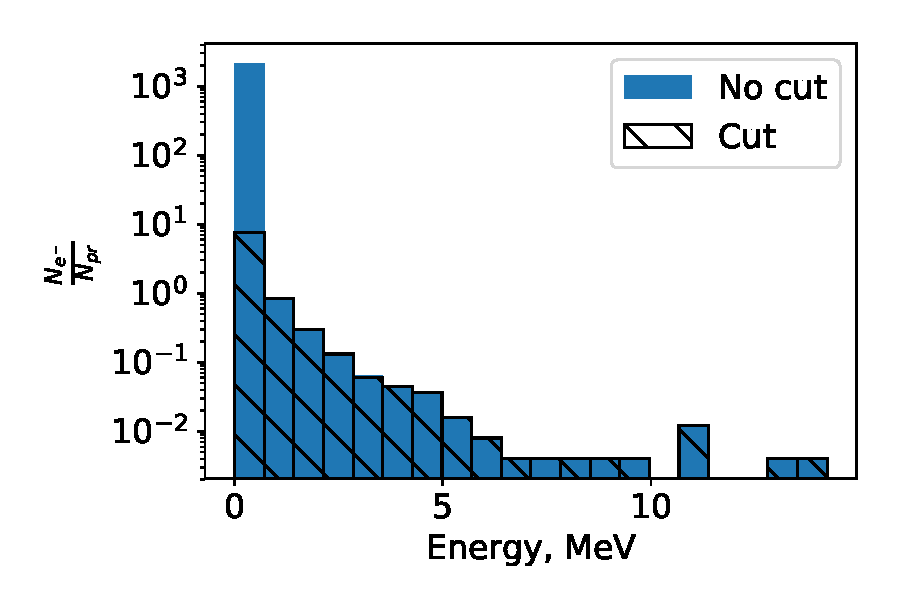
\includegraphics[width=0.95\linewidth]{pictures/06_energy_cut_electron}
    %         \caption{}
    %         \label{pic-electron-cut-a}
    %     \end{subfigure}
    % 	~
    %     \begin{subfigure}[b]{0.5\textwidth}
    % 		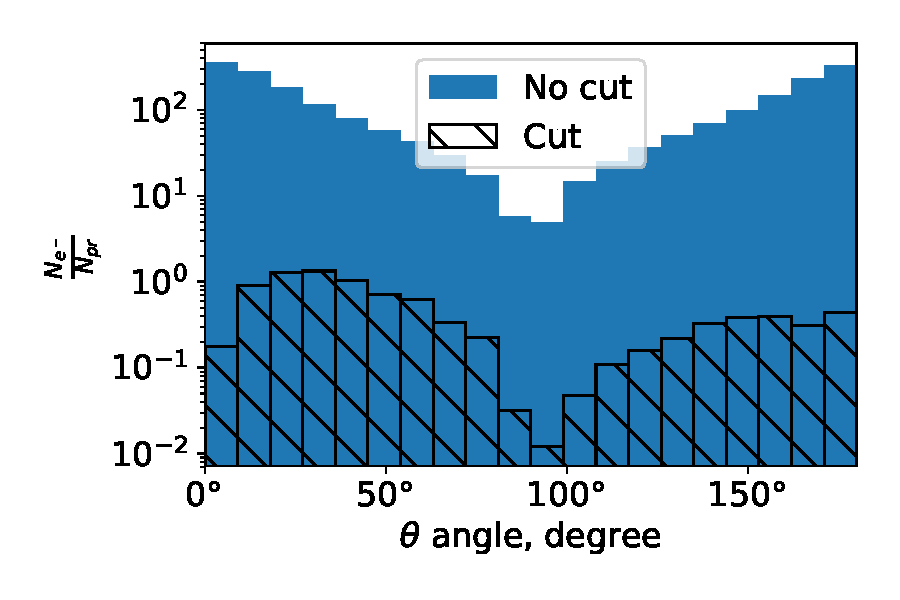
\includegraphics[width=0.95\textwidth]{pictures/07_theta_cut_electron}
    %         \caption{}
    %         \label{pic-electron-cut-b}
    %     \end{subfigure}
    %     \caption{ a) Energy b) polar angle secondary electron distribution after and before cut for next parameters: primary electron energy - 1 MeV, field area size - 400 meter, electric field 1.5 kV/cm, air density - $0.3 kg/m^3$ ($\sim 0.2 atm$)}
    % \end{figure}
    
    % On Fig.~\ref{pic-positron-cut-a} and ~\ref{pic-positron-cut-b} show spectrum of positron after and before involving selection rules. Similar spectrum with another set of simulation parameters for secondary 
    % % \todo{кто такие третьи електроны вообще не понятно. З. поправил} 
    % electrons shown on Fig.~\ref{pic-electron-cut-a} and \ref{pic-electron-cut-b}
    
    % \begin{figure}[ht!]
    % \begin{center}
    % 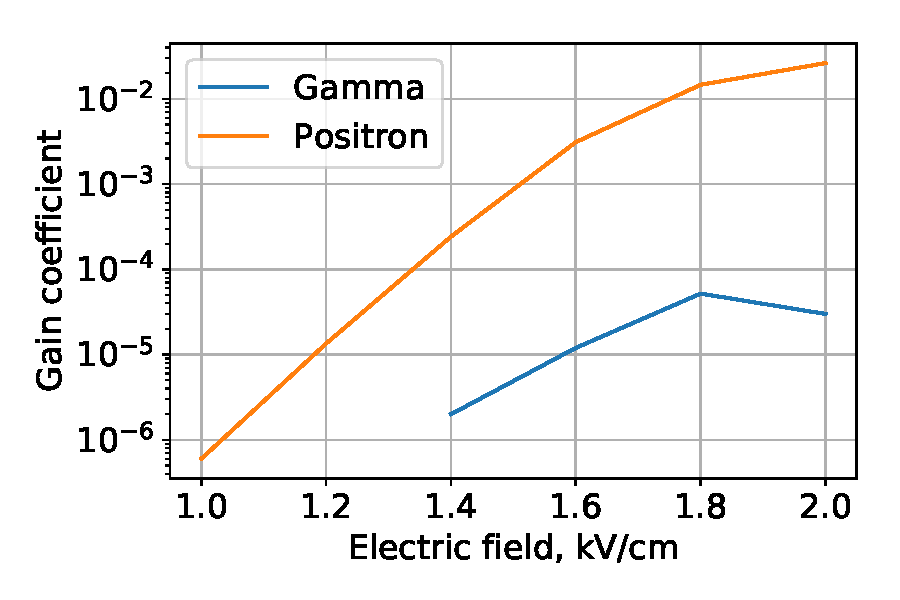
\includegraphics[width=0.5\linewidth]{pictures/08_gain}
    %         \label{pic-gain-a}
    %          \caption{Positron (gamma) feedback coefficient dependent on cell electric field for next parameters: primary electron energy - 3 MeV, field area size - 400 meter, electric field from 1 to 2 kV/cm, air density - $0.5 kg/m^3$ ($\sim 0.5 atm$)}
    % \end{center}
    
    %    \end{figure}
    
    % \begin{figure}[ht!]
    % 	\begin{subfigure}[b]{0.5\textwidth}
    %     	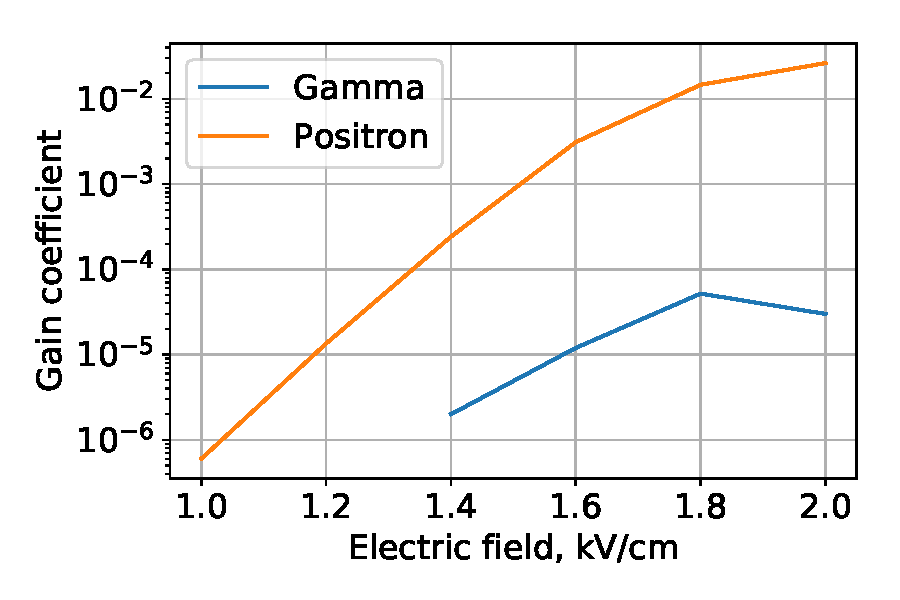
\includegraphics[width=0.95\linewidth]{pictures/08_gain}
    %         \caption{}
    %         \label{pic-gain-a}
    %     \end{subfigure}
    % 	~
    %     \begin{subfigure}[b]{0.5\textwidth}
    % 		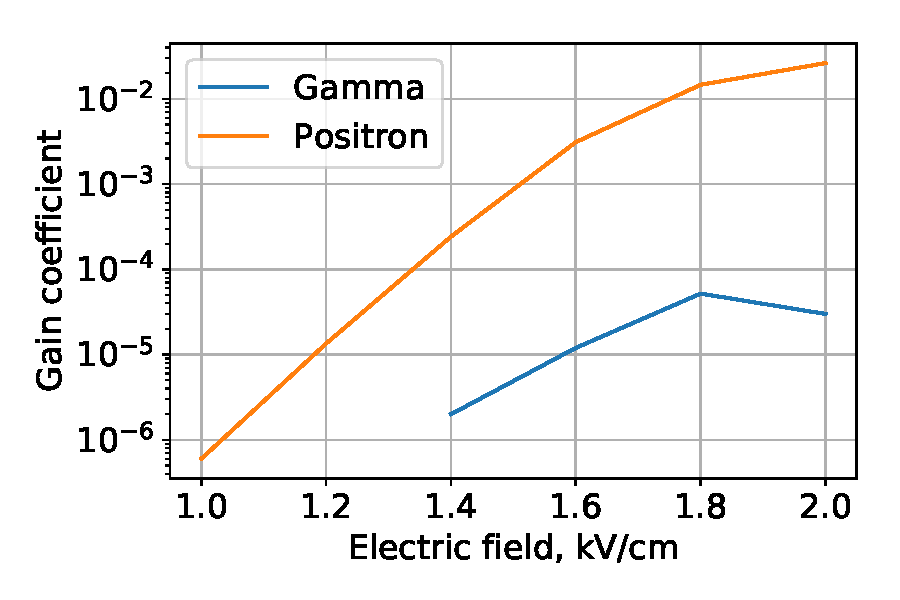
\includegraphics[width=0.95\textwidth]{pictures/08_gain}
    %         \caption{}
    %         \label{pic-dwayer-b}
    %     \end{subfigure}
    %     \caption{a) Positron (gamma) feedback coefficient dependent on cell electric field for next parameters: primary electron energy - 3 MeV, field area size - 400 meter, electric field from 1 to 2 kV/cm, air density - $0.5 kg/m^3$ ($\sim 0.5 atm$)
    % %     b) Dwyer model in Geant 4 simulation. Red tracks – electrons. Blue tracks – positrons. Green tracks - gamma-rays
    % }
    % \end{figure}
    
    %The result of simulations is significantly different from Dwyer results. But by reason of high computing difficult Monte-Carlo simulation, we used several approximation, which inevitably influence on result precision. 
    
    The gain coefficient is calculated as a convolution of probabilities of producing valid particle on each step and applying all relevant cuts.
    
    Using simulation result we calculate gain coefficient by previously introduced formula. The result for general cell geometry (\todo{which conditions}) is presented at Fig.~\ref{pic-gain-a}. It could be clearly seen that the total gain factor is significantly smaller than one for fields smaller than 200 kV/m. The gamma gain negligible and positron gain tops at about 6\%. Such small number could not explain self-sustaining discharge mechanism, proposed by Dwyer and give only small contribution to total charge generation.
    
    One should note, that Dwyer mechanism could still work for higher fields (like 1000 kV/m), but those conditions are unreachable for both real gas and simulations, because normal gas breakdown in moist (and even dry) air starts much sooner. Experimental evidence shows that it is not the case in thunderclouds.
    
    The model shows a positron annihilation line in gamma-spectrum, which was observed in multiple experiments (\todo{link to nature article}). This line is an intrinsic part of any model based on Gurevitch runaway model, still this positron line does not guarantee the role of positrons in producing the feedback. Detailed numerical estimation of those effects requires additional simulation with enhanced statistics which is being performed right now.
    
    %The results above are obtained with some assumptions. 
    %Я раз пять прочитал, но все равно не понял, что тут написано 
    %З. Я пишу от том что мы использовали всякие приближения, но делали этот так что бы получить верхнюю оценку коээфициента усиления, условие разворота не учитывает рассеяние электронов, которое вообще говоря сильно влияет позволя электроно с над критичиским углами разоврачиваться, но посколькку оно мешает разворачиваться электронам способным на это, то в среднем можно считать что оно не мешает. Затем я говорю что статистика маленькая и сейчас проводится более точное моделирование
    %Although we leaded to choose approximation setting upper estimation of gain coefficient, this aim can't always be achieved. So for calculation of critical angle of reverse don't take to consideration elastic scattering, due to which several electron can turn at angles greater that critical angle. But analogy electron capable of reverse will be stopped by electric field, because we could take what procedure of selection by critical angle is right on average. Same exist necessary in increase of simulation statistics. Nevertheless getting estimation show what couldn't confidently affirm about strong influence positron (gamma) feedback mechanism on process in thunderstorm and. At the present time, we make precision Monte-Carlo simulation for getting final answer.
    
    \section{Conclusion}
    
    The results of GEANT4 simulations, presented in this article clearly show that positron and gamma feedback introduces very small (few percents at most) contribution to total charge generation in the thundercloud under realistic conditions (electric field between 100 and 250 kV/m and pressure from 0.5 to 0.8 atmosphere). 
    
    Dwyer positron enhancement is still possible for much higher electric fields (like 1000 kV/m), but those fields are unreachable in the thunderclouds since they are higher than the breakdown field. The simultaneous increase of field and density proposed in one of works by Dwyer(~\cite{dwyer2003fundamental}) conserves Gurevitch's critical energy but strongly affects the number of produced positrons (both changes work in direction of increasing positron flux).
    
    %The paper presents a study of relativistic electron avalanches in cells with air density characteristic for atmosphere heights where clouds are formed and electric field value between 1 and 2.5 kV/cm. The result shows that positron gain coefficient in such cells is less than 0.01. Consequently, Dwyer feedback occurs rarely to increase runaway electron flux significantly.
    % То, что ниже ниоткуда не следует
    %The conditions when positron feedback coefficient is equal one were not determined. Nevertheless, Dwyer’s conditions~\cite{dwyer2003fundamental} were checked. In such conditions infinite electron avalanche reproduction works. However, the study shows that new electron avalanche models are needed to describe thunderstorm processes.
    
    This work is supported by the Russian Science Foundation under grant No. 17-12-01439.
    %This work is supported by the Ministry of Education and Science of the Russian Federation under the contract No. 3.3008.2017/PP.
    
    \bibliography{references}{}
\end{document}
